\graphicspath{{chapters/04/}}
\chapter{Approximation algorithms}

Can we assume that in any condition the stochastic simulation bottleneck
is a problem? It depends. If we are in a condition in which all species
are present in low number and it takes a lot to cure, the stochastic
simulation is not really a bottleneck. We might have an issue if we wish
to simulate for a long time, multiplicative factors. At the moment, it
is not feasible to compute exact a stochastic simulations to all the
models we need to observe, in particular for huge number of species and
reaction, therefore there is a huge research in developing alternative
strategies that allow to compute the system in an \emph{accurate} way
(lose correctness) with lower computational cost and time.

Why should we decide to use approximations in simulations?

\begin{enumerate}
\def\labelenumi{\arabic{enumi}.}
\tightlist
\item
  it might be the only possible and feasible solution to solve a
  problem.
\item
  reality is affected by error, so even when we are using exact
  stochastic simulation algorithms we should consider a small degree of
  approximation. A certain deal of error could aid in retrieving a more
  realistic result.
\end{enumerate}

In chapter 3 all the algorithms were belonging to exact stochastic
simulation setting, so the result is the same. Instead in this case,
each algorithm approximates in a different way, assume different
approximation → not a consistent set.

We should observe that of the three main computational strategies
presented here, there is one which is much more popular with respect to
other. The $\tau$ leaping method is well known and has been further
developed, so we will be focusing on it.

\begin{figure}
\centering
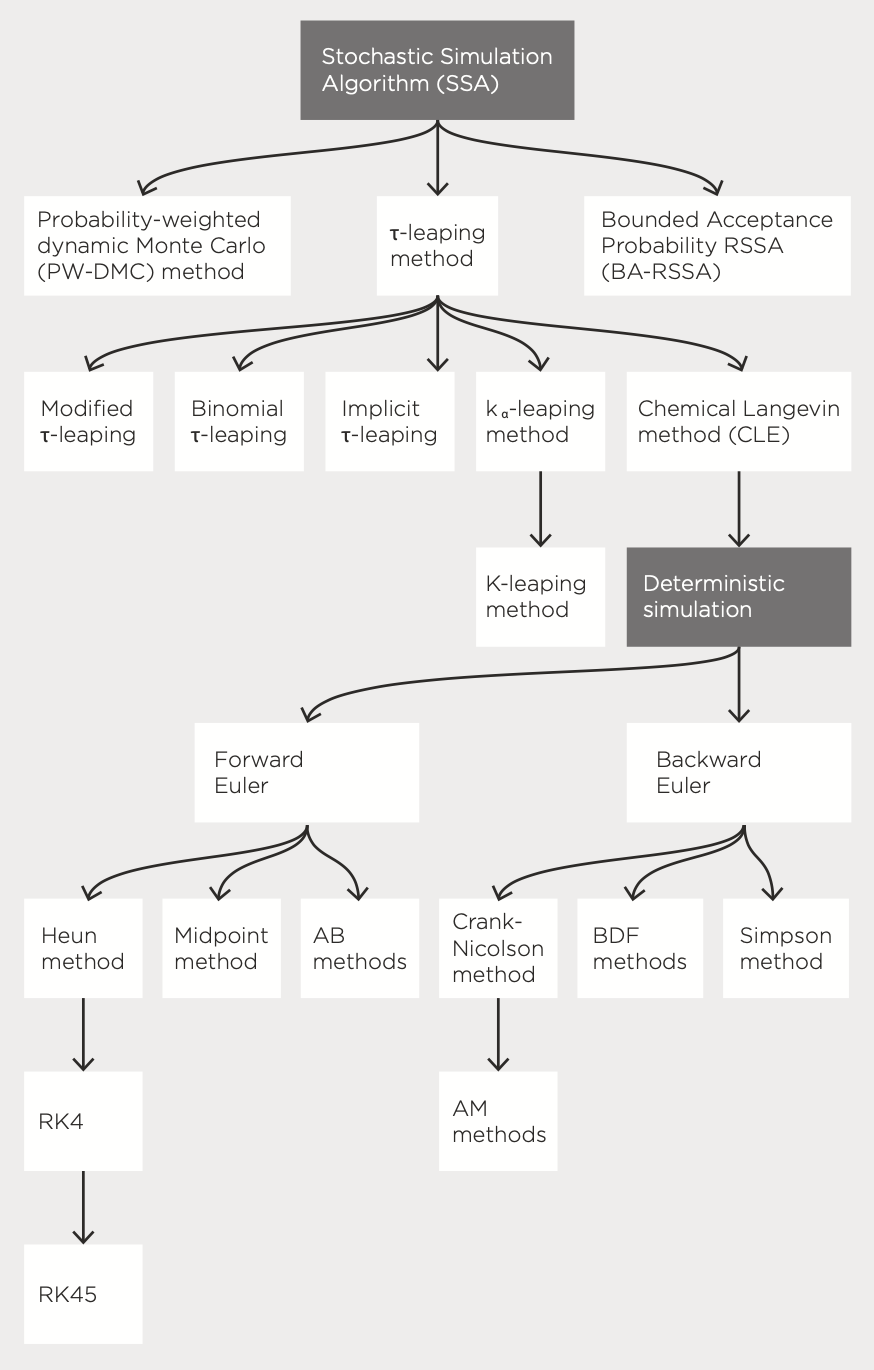
\includegraphics{04_images/SSA_tree.png}
\end{figure}

Before introducing the algorithm, let's try to think about the possible
bottlenecks which could prevent us from having a fast algorithm. We
could improve:

\begin{itemize}
\tightlist
\item
  work on the number of reaction events, group them in such a way to
  reduce the number of reactions in the system. The $\tau$ leaping
  methodology is working in this direction
\item
  improve the computation of the propensity. For instance, the
  probability-weighted Monte Carlo is particularly promising in
  situations in which we have huge differences in propensities among
  reactions.
\end{itemize}

\hypertarget{probability-weighted-dynamic-monte-carlo-method}{%
\section{\texorpdfstring{\textbf{Probability-Weighted Dynamic Monte
Carlo
Method}}{Probability-Weighted Dynamic Monte Carlo Method}}\label{probability-weighted-dynamic-monte-carlo-method}}

The probability-weighted dynamic Monte Carlo method (PW-DMC) is an
approximation approach for improving computational efficiency of
stochastic simulation of reaction networks where some reactions have
propensities significantly larger than other reactions. The principle of
this algorithm is a sort of modification of the probability distribution
NRM through \emph{weighted sampling}. The idea is to introduce a bias
weight value on the propensity, in order to take into the account the
number of times in which the reaction is executed. We will have a lower
amount of iterations at the price of applying reactions a different
number of times according to the probability.

The weight is a multiplicative factor of the stoichiometric coefficient.
$\mu$ is the smallest reaction index $\mu$ such that:

$$
\sum^{\mu}_{j=1} a^w_j \geq r_1 a^w_0 
$$

Second, PW-DMC has to correct the firing time $\tau$ of reaction $R_\mu$
because it is selected through the weighted sampling. The generation of
$\tau$ is adapted from SSA in which it is generated from an exponential
distribution with rate $a^w_0$. PW-DMC then updates the state at time
$t + \tau$ by assuming that there are $w_\mu$ consecutive firings of $R_\mu$ in
the time interval $[t,t + \tau)$.

This methodology started to provide some hints for the approximation
setting. In the complete algorithm we have the concept of effective
propensity, allowing to reach the speed up.

\hypertarget{bounded-acceptance-probability-rssa}{%
\section{Bounded Acceptance Probability
RSSA}\label{bounded-acceptance-probability-rssa}}

If we compare RSSA and DM algorithm, the main difference is that the
RSSA algorithm is more complex than DM at each iteration. The bottleneck
in RSSA is that we use the third random numbers for the rejection test,
so this algorithm tries to speed up the process and reduce the
complexity. If we decide to accept everything, we will end up with a
strong bias. In order to avoid the high computational costs, we can only
apply rejection to some cases → set up bounds, reaching bounded
acceptance probability RSSA. If the probability of the candidate
reaction is greater than certain amount, we accept it without the
rejection test.

Algorithm: we are still executing one reaction at a time. Comparing in
terms of accuracy, the approximation of the previous method is not
applied. Here we are not working with the real propensity. In this
version we are totally avoiding the rejection-based part, the
approximation in this case increases the error. It could be possible to
apply a strategy in which we apply rejection based only in certain
conditions (more complex).

By looking at the literature, it is interesting to rank strategies in
terms of accuracy and time.

\hypertarget{tau-leaping-method}{%
\section{\texorpdfstring{$\tau$-Leaping
Method}{-Leaping Method}}\label{tau-leaping-method}}

The $\tau$-leaping method is a stochastic approximate algorithm for
improving performance of stochastic simulation. Its aim is to discretize
the time axis into time intervals and to approximate the number of
reactions firing in each time interval. The simulation then leaps from
one time interval to the next interval with many reaction firings
performed simultaneously.

What is remarkable here, is that we are doing an approximation over the
number of iterations which is much more relevant than previous
approaches. We are grouping a mixture of events, which can be defined as
a \emph{macrostep}. If $\tau$ is big, the number of iterations will be
low and the complexity will decrease. We should constraint the error in
such a way that we are aware of its value as a constant.

Which could be a high-level property of tau to apply macrostep without a
crude error in the simulation? We should impose certain logics on $\tau$.

{[}lo schermo non va{]}

``vabbè, let me see. Ragazzi non facciamo più niente, nel senso, cosa
devo fare?Sono arrabbiatino!\ldots{[}funziona{]} La forza? It's possible
that? Ahahah''

We want to limit the bias on the propensity. This translates in tau
selection satisfying the so-called ``\textbf{leap condition}'':

There exists a leap $\tau > 0$ such that the change in propensity $a_j$ of
each reaction $R_j$ with $j = 1,...,M$ during the time interval
$[t,t +\tau)$ is negligibly small.

Negligibly small means lower than some threshold. By applying a proper
reasoning we reach the following formula, in which we derive the update
of the state. Once we have selected $\tau$, we will evolve the system by
adding to he current state a certain amount of firing for each one of
the reactions in the system {[}for each reaction j from 1 to m we apply
a certain amount of time{]}.

$$
                X(t+\tau)=\mathbf{x}+\sum_{j=1}^{M}k_j\mathbf{v}_j =\mathbf{x}+\sum_{j=1}^{M}Poi(a_j(x)\tau)\mathbf{v}_j         
$$

$k_j$ will be generated through a Poisson distribution, which will
depend over the specific propensity multiplied by the size of the step.
The algorithm is applying any of the reactions per a specific amount of
time.

Pros: we are allowed to work with higher $\tau$ with respect to exact
stochastic simulations.

Cons: if we only have rare events, the algorithm will not be the best
solution (as it will try to apply all reactions at all the times). Given
however that in any system there are at least some reactions with high
propensity, at the very end we still gain a huge speed-up.

\hypertarget{choosing-tau---leap-selection-section}{%
\subsection{Choosing tau - Leap selection
section}\label{choosing-tau---leap-selection-section}}

\hypertarget{postleap-tau-selection}{%
\subsubsection{\texorpdfstring{\textbf{Postleap $\tau$
Selection}}{Postleap  Selection}}\label{postleap-tau-selection}}

Choose a $\tau$ from a Poisson distribution and see if it is fine for
the simulation. We start from a predefined arbitrary $\tau$ (small),
then we have a trial procedure. The algorithm will compare the
difference in the propensity before and after, to assess whether $\tau$
is of the right size. E.g. if the change in propensity is small, we can
use a greater $\tau$.

The complexity of the $\tau$-leaping is moved to a sub-problem, which is
the choice of $\tau$ . We could also perform a preleap selection or
choose other strategies.

The Poisson distribution could provide more events than the ones that
are possible in the system; in this case we end up with a negative
population. While performing $\tau$-leaping, we will need to make sure
that a negative scenario is never reached through a test. The real
amount of time executing k should be computed as the mean from k
generated from Poisson distribution and the availability of the
reactants {[}non chiaro{]}.

We can bridge $\tau$-leaping with exact stochastic simulation when we
have only rare events

\hypertarget{chemical-langevin-method}{%
\section{\texorpdfstring{\textbf{Chemical Langevin
Method}}{Chemical Langevin Method}}\label{chemical-langevin-method}}

We can use the Normal distribution instead of Poisson, and scale it with
mean and variance with another Normal formula based on a (0,1)
distribution, obtaining a simplified method. We will not have main
events, but main \emph{drivers} in the system. Stochasticity is strongly
approximated, we are moving to an idea of average, real numbers. This
will be the starting point for the deterministic simulation.

\textbf{COPASI} is a well-known simulator. It exploits Gillespie's
algorithm and $\tau$-leaping algorithm. IN general, any simulator offers
many algorithms, so we should be able to choose the best computational
approach → calibrating the model. The stochastic rate provides us the
speed, we require to derive it with some methods; all simulations
algorithm compute deterministically or stochastically a speed for the
reaction, computed over parameters of the model e.g.~the rates. The
rates, as the initial values, are not free-lunch, they can be derived
through experiments.

Often times, we work with models with not fully known parameters; in the
second module we will explore solutions for \emph{estimating the
parameters} (reverse engineering approach).

During the last lecture, we focused on $\tau$-leaping.
\textbf{\emph{Adaptive algorithms}} select a delta and change it
adaptively during the simulation in order to reach the best results, for
instance post leap $\tau$ selection.

\textbf{Chemical Langevin Method} allows to modify the evolution of the
system; the update formula depends on the propensity, but allows to
distinguish a totally deterministic part from the stochastic one. This
algorithm also has an important difference with previously seen
strategies: we do not have integers, we will be provided with a real
number adding some noise. This dynamics is over continuous numbers,
tends to an average behaviour.
